\subsection{Use Cases}
\begin{figure}[!htbp]
\centering
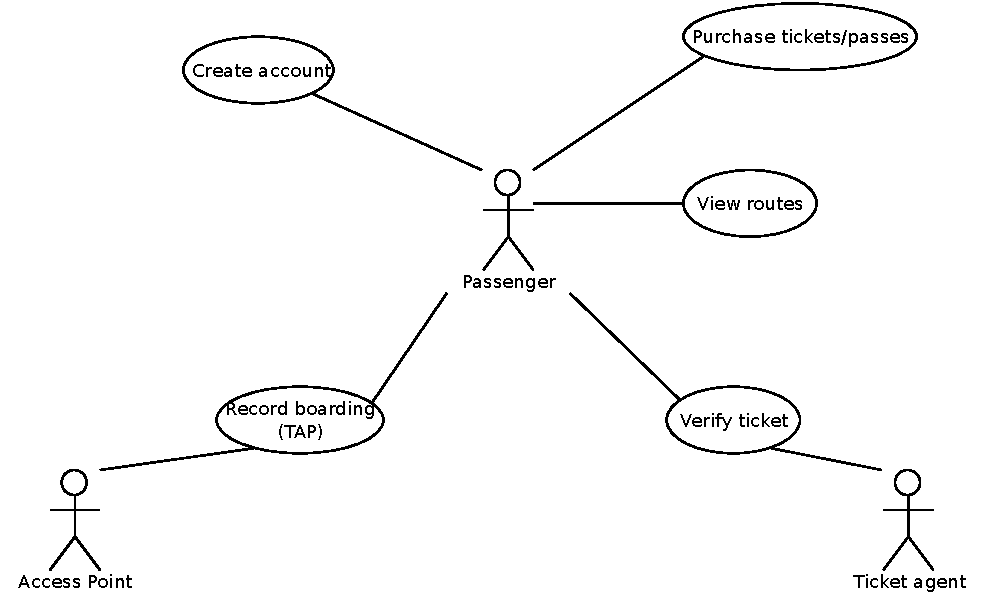
\includegraphics[width=0.7\textwidth]{arch/usecase.pdf}
\end{figure}

The basic use scenarios are:\begin{description}
\item[Account creation] The user can create accounts from within the app.
\item[View routes] Upon locating the user via GPS, the app presents a list of nearby routes.
\item[Purchase of tickets/passes	] The user may purchase a pass, or simply add money to their TAP funds.
\item[Record boarding] Upon boarding the train/bus, the user must record this by presenting the QR code to the turnstile/bus driver.
\item[Ticket verification] A ticket agent aboard a train/bus may ask passengers to present proof of payment at any time. This is again verified by a QR code.
\end{description}

\clearpage

\subsection{Class Hierarchy}
\begin{figure}[!htbp]
\centering
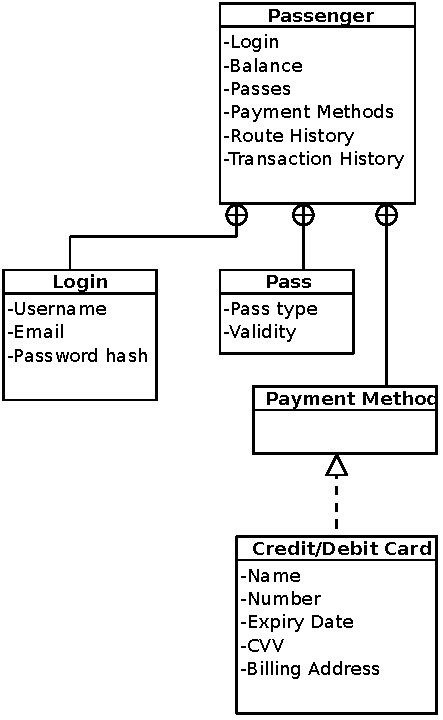
\includegraphics[width=0.5\textwidth]{arch/classdiagram.pdf}
\end{figure}

The important classes to be maintained are:\begin{description}
\item[Passenger] Maintains passenger data such as login info and payment history.
\item[Login] Holds a username paired with a password that is hashed for security.
\item[Passes] Maintains the list of fare payment methods available to the passenger. Also selects the most appropriate one for each journey (Eg. If a passenger has a day pass then fare will not be deducted from TAP funds.)
\item[Payment Methods] An abstraction for various payment methods. This layer allows addition of functionality in the future, eg. Google Wallet and Paypal.
\end{description}

\subsection{Software Choices}
\begin{description}
\item[PhoneGap] We chose PhoneGap as our development platform primarily due to the cross-compatibility it provided.Further, applications on PhoneGap can be built out of web technologies that our team is already familiar with.
\item[Fluid UI] Fluid UI was chosen as a prototyping tool due to its ability to iteratively generate prototypes.
\item[Oracle Database] We primarily chose Oracle Database because it is the current database solution emplyed by TAP. Because it is vital that our mock databases be eventually compatible with existing infrastructure, we chose to use their selections.
\item[Siebel Web Interface] We chose the Siebel interface for the same reasons as above.
\item[Metro API] We use the Metro API to retreive transit information as well as travel alerts.
\end{description}